\vspace{10pt}

{\centering\subsection*{白水:如何写读书笔记?}}

\addcontentsline{toc}{subsection}{白水:如何写读书笔记?}

\renewcommand{\leftmark}{白水:如何写读书笔记?}

\begin{figure}[htbp]

\centering

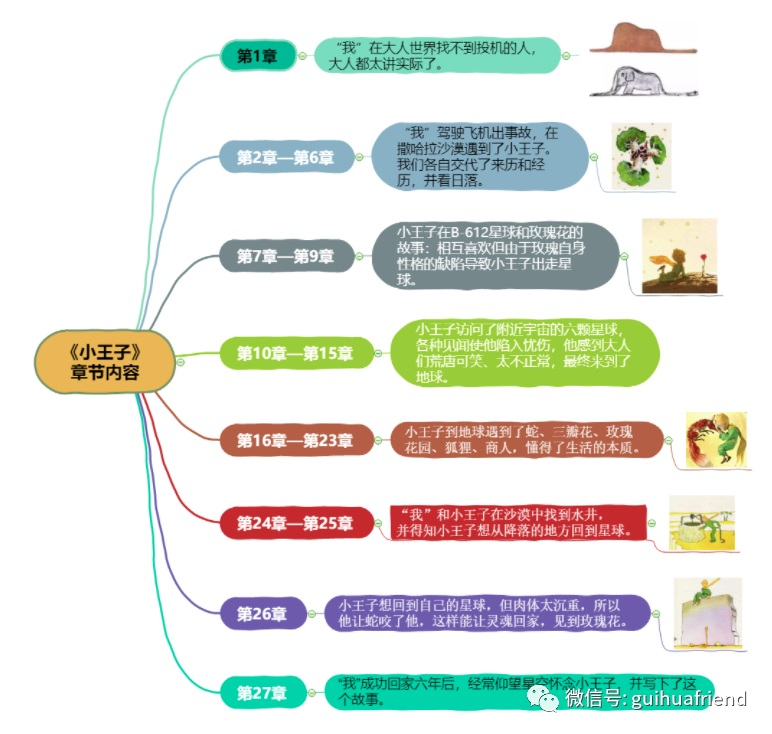
\includegraphics[width = .5\textwidth]{./ch/v7.jpg}

\end{figure}


与你共同成长。



你好,这里是桂花图书馆写作分享,我是馆长莫静琴。



上周龙柏泉的分享聊到“如何写一个好的故事”。除了故事的六要素之外,柏泉还谈到了写好一个故事也要结合自身经历,从小事入手,以及从旁观者获得反馈和列提纲。那么,如果我们阅读一本有故事情节的书之后,如何写读书笔记呢?



首先,如何发现值得精读和写读书笔记的书?



如果我们通过大量的浏览和快速阅读,发现一些非常感兴趣的书。并且这些书正好也非常经典,获得很多爱读书的人的推荐和好评,那么这些书就非常值得精细阅读,甚至值得写读书笔记。例如阅读专家推荐的书,重要的图书排行榜,获奖书籍都是不错的好书来源。例如担当者计划班班有个图书角的书单,爱阅公益的年度书单等。







再者,为何要写读书笔记?



好记忆不如烂笔头。读书笔记可以作为一本书的浓缩版,相当于提取出了书里面的核心或者精华内容。我们下次再看读书笔记,可以快速的获知一本书的内容。写读书笔记是一种主动的阅读方法,也是一种高效的精读方式。当我们带着目标去阅读的时候,可以提高阅读效率,练习寻找最重要的、最核心的或最关心的信息的能力。读书笔记也可以帮助我们梳理书的内容,练习复述能力。复述一本书的主要内容,相当于一个自我的反馈和测试过程。有了这个过程,我们才能知道自己对一本书的理解程度,是不是还需要多读几遍。



最后,写读书笔记有哪些方法?



可以带着一些问题去阅读去构思。例如,有哪几个重要的人物,人物之间的关系和性格特点,主要的故事情节,故事的背景等等。甚至可以画一画人物关系图等。可以摘抄书里面让自己受到启发的句子,也可以思考,这本书给了自己哪些启发。甚至能不能通过书里面的观点来分析自己的经历。例如,《小王子》里面说“你在你的玫瑰花身上耗费的时间使得你的玫瑰花变得如此重要。” 这让我们体会到,一个人或者一件东西对一个人的重要性,在于投入的时间多少。我们最要好的朋友是谁,是不是那些愿意花时间陪伴我们的人。假如一个兴趣对我们很重要,比如下棋啊,钓鱼啊,阅读啊,是不是因为我们愿意投入和已经投入了很多时间。






这是我们这周的分享。谢谢大家。

\vspace{10pt}

文稿:白水

朗读:莫静琴

发布:2021年5月22日







\vspace{10pt}

\hline

